\documentclass[11pt, a4paper]{article}
\usepackage[utf8]{inputenc}
\usepackage{geometry}
\usepackage{graphicx}
\usepackage[dvipsnames]{xcolor}
\geometry{margin=1in}
\setlength{\parindent}{0em}
\setlength{\parskip}{1em}
\title{Computação Gráfica | Trabalho 1}
\author{Professor: Waldemar Celles\\
Aluno: Antenor Barros Leal}
\date{29 de setembro de 2024}
\begin{document}
\maketitle

\section {Resumo}
Este trabalho tem como objetivo fazer uma representação simplificada do sistema 
solar, onde são mostrados o Sol, Mercúrio, a Terra e a Lua. A simulação 
usa transformações, texturas dentro de uma hierarquia de nodes que organiza os
movimentos de cena permitindo ser possível movimentos compostos como da Lua em
torno da Terra e, ao mesmo tempo, do Sol.

\section {Escalas e períodos}

As escalas e distâncias dos planetas em relação ao Sol não são realistas, pois, 
para isso, os planetas teriam que ser muito pequenos e distantes um do outro, 
tornando-os difíceis de visualizar. Entretanto, as relações entre os períodos 
orbitais são realistas.

Na classe da engine, vemos um valor padrão de 1/365, representando o período 
orbital da Terra em dias. Multiplicamos por 5000 para que o movimento fique 
perceptível e multiplicamos por \texttt{dt} (o intervalo de tempo entre 
chamadas da função \texttt{update}) para que o movimento seja agnóstico em 
relação à velocidade do computador. A seguir o código da função update.

\begin{verbatim}
virtual void Update (float dt)
{
    m_trf->Rotate(dt * 5000 / m_period, 0, 0, 1);
}
\end{verbatim}

Para a rotação da Terra (transformação \texttt{earthOrbit}), usei o valor 10. 
Embora isso não seja realista (o certo seria 1), foi necessário utilizar um 
valor mais alto para que o movimento de rotação da Terra não ficasse extremamente 
rápido.

\section {Diagrama}

O diagrama a seguir apresenta o grafo de cena, mostrando os objetos criados e 
suas conexões hierárquicas.

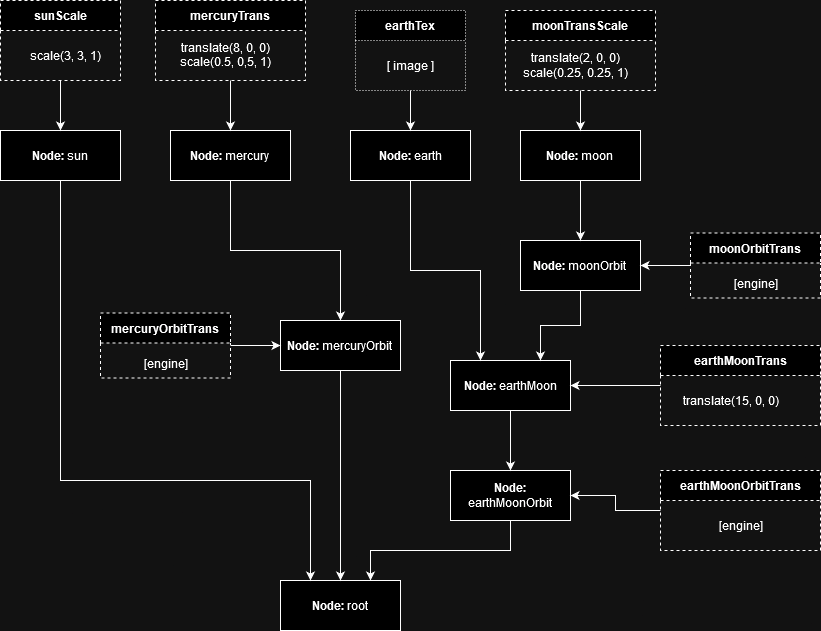
\includegraphics[width=\linewidth]{Trab1Graph.png}

\section {Nodes e Transformações}

Os planetas e o Sol são representados por formas primitivas do tipo 
\texttt{Disk}, instanciadas nos nodes \texttt{sun}, \texttt{mercury}, 
\texttt{earth} e \texttt{moon}. Abaixo, o papel de cada node e suas 
respectivas transformações:

\subsection{Sol}
O node \texttt{sun} contém a transformação \texttt{sunScale}, que ajusta o 
tamanho e a posição do Sol. Esta transformação é usada para centralizar o Sol e 
mudar seu tamanho.

\subsection{Mercúrio}
O node \texttt{mercury} contém a transformação \texttt{mercuryTrans}, responsável 
por posicionar Mercúrio em sua órbita em torno do Sol. Ele é escalado para ser 
menor que a Terra e o Sol. O node \texttt{mercuryOrbit} envolve Mercúrio, 
servindo para rotacioná-lo em torno do Sol. Este node é controlado pelo
\texttt{mercuryOrbitTrans}, que atualiza sua rotação com base no período da 
órbita de Mercúrio (88 dias, aproximadamente).

\subsection{Terra e Lua}
O node \texttt{earth} contém a transformação \texttt{earthOrbit}, que faz a 
Terra girar em torno dela mesma. Para a Lua, temos dois nodes de transformação:

\begin{itemize}
\item \texttt{moonTransScale}: responsável por posicionar a Lua em relação à Terra, 
ajustando sua escala e distância.
\item \texttt{moonOrbit}: é um "container" que faz a Lua orbitar a Terra. Se
aplicassemos o engine diretamente no moon, a Lua rotacionaria em 
torno de si mesma, em vez de orbitar a Terra.
\end{itemize}

O node \texttt{earthMoon} agrupa a Terra e a Lua, permitindo que ambas sejam 
posicionadas como um sistema em torno do Sol. Já o node 
\texttt{earthMoonOrbitTrans} é responsável pela rotação do sistema Terra-Lua em 
torno do Sol.

\subsection{Espaço}
O fundo da cena é representado por uma textura estrelada, aplicada a um quadrado 
escalado (primitiva \texttt{Square}). A transformação \texttt{spaceTrans} ajusta 
o tamanho e a posição desse quadrado para ocupar todo o plano de fundo. Para 
garantir que o fundo fique atrás dos planetas e do Sol, a componente \texttt{z} 
da transformação de escala é ajustada para um valor inferior, zero, no caso,
enquanto todos os outros ficam com z igual a um.

\section {Composição de Cena}

A cena completa é composta pela árvore de nodes descrita acima:

\begin{itemize}
\item O \texttt{root} contém os nodes do Sol, Mercúrio e o sistema Terra-Lua, além 
do fundo.
\item As engines de movimentação (\texttt{MovePointer}) são responsáveis por 
atualizar as órbitas com base no tempo.
\end{itemize}

Essa composição hierárquica permite que a simulação funcione de maneira modular, 
onde cada corpo celeste tem suas transformações e atualizações associadas à sua 
posição local e movimento dentro do sistema solar.

\end{document}